\documentclass[10pt,a4paper,onecolumn]{article}
% \usepackage[utf8]{inputenc}
\usepackage{marginnote}
\usepackage{amssymb,amsmath}
\usepackage{graphicx}
\usepackage{xcolor}
\usepackage{authblk,etoolbox}
\usepackage{titlesec}
\usepackage{calc}
\usepackage{hyperref}
\hypersetup{breaklinks=true,
            bookmarks=true,
            pdfauthor=
{
      Timothée Poisot,
  },
            pdftitle=
{
[Re] On the coexistence of specialists and generalists
},
            colorlinks=true,
            citecolor=blue,
            urlcolor=blue,
            linkcolor=blue,
            pdfborder={0 0 0}}
\urlstyle{same}
\usepackage{tcolorbox}
\usepackage{ragged2e}
\usepackage{fontspec}
\usepackage{fontawesome}
\usepackage{caption}
\usepackage{listings}
\lstnewenvironment{code}{\lstset{language=Haskell,basicstyle=\small\ttfamily}}{}



%\usepackage{fancyvrb}
%\VerbatimFootnotes
%\usepackage{graphicx}
%\usepackage{mdframed}
%\newmdenv[backgroundcolor=lightgray]{Shaded}


\usepackage{longtable,booktabs}

\usepackage[
  backend=biber,
%  style=alphabetic,
%  citestyle=numeric
]{biblatex}
\bibliography{bibliography.bib}



% --- Macros ------------------------------------------------------------------
\renewcommand*{\bibfont}{\small \sffamily}

\definecolor{red}{HTML}{CF232B}
\newcommand{\ReScience}{Re{\bfseries \textcolor{red}{Science}}}

\newtcolorbox{rebox}
   {colback=blue!5!white, colframe=blue!40!white,
     boxrule=0.5pt, arc=2pt, fonttitle=\sffamily\scshape\bfseries,
     left=6pt, right=20pt, top=6pt, bottom=6pt}

\newtcolorbox{repobox}
   {colback=red, colframe=red!75!black,
     boxrule=0.5pt, arc=2pt, left=6pt, right=6pt, top=3pt, bottom=3pt}

% fix for pandoc 1.14
\newcommand{\tightlist}{%
  \setlength{\itemsep}{1pt}\setlength{\parskip}{0pt}\setlength{\parsep}{0pt}}

% --- Style -------------------------------------------------------------------
\renewcommand*{\bibfont}{\small \sffamily}
\renewcommand{\captionfont}{\small\sffamily}
\renewcommand{\captionlabelfont}{\bfseries}

\makeatletter
\renewcommand\@biblabel[1]{{\bf #1.}}
\makeatother

% --- Page layout -------------------------------------------------------------
\usepackage[top=3.5cm, bottom=3cm, right=1.5cm, left=1.5cm,
            headheight=2.2cm, reversemp, includemp, marginparwidth=4.5cm]{geometry}

% --- Section/SubSection/SubSubSection ----------------------------------------
\titleformat{\section}
  {\normalfont\sffamily\Large\bfseries}
  {}{0pt}{}
\titleformat{\subsection}
  {\normalfont\sffamily\large\bfseries}
  {}{0pt}{}
\titleformat{\subsubsection}
  {\normalfont\sffamily\bfseries}
  {}{0pt}{}
\titleformat*{\paragraph}
  {\sffamily\normalsize}


% --- Header / Footer ---------------------------------------------------------
\usepackage{fancyhdr}
\pagestyle{fancy}
%\renewcommand{\headrulewidth}{0.50pt}
\renewcommand{\headrulewidth}{0pt}
\fancyhead[L]{\hspace{-1cm}
\includegraphics[width=4.0cm]{rescience-logo.pdf}}
\fancyhead[C]{}
\fancyhead[R]{}
\renewcommand{\footrulewidth}{0.25pt}

\fancyfoot[L]{\hypersetup{urlcolor=red}
              \sffamily \ReScience~$\vert$
              \href{http://rescience.github.io}{rescience.github.io}
              \hypersetup{urlcolor=blue}}
\fancyfoot[C]{\sffamily 1 - \thepage}
\fancyfoot[R]{\sffamily Sep 2015 $\vert$
                        Volume \textbf{1} $\vert$
                        Issue \textbf{1}}
\pagestyle{fancy}
\makeatletter
\let\ps@plain\ps@fancy
\fancyheadoffset[L]{4.5cm}
\fancyfootoffset[L]{4.5cm}

% --- Title / Authors ---------------------------------------------------------
% patch \maketitle so that it doesn't center
\patchcmd{\@maketitle}{center}{flushleft}{}{}
\patchcmd{\@maketitle}{center}{flushleft}{}{}
% patch \maketitle so that the font size for the title is normal
\patchcmd{\@maketitle}{\LARGE}{\LARGE\sffamily}{}{}
% patch the patch by authblk so that the author block is flush left
\def\maketitle{{%
  \renewenvironment{tabular}[2][]
    {\begin{flushleft}}
    {\end{flushleft}}
  \AB@maketitle}}
\makeatletter
\renewcommand\AB@affilsepx{ \protect\Affilfont}
%\renewcommand\AB@affilnote[1]{{\bfseries #1}\hspace{2pt}}
\renewcommand\AB@affilnote[1]{{\bfseries #1}\hspace{3pt}}
\makeatother
\renewcommand\Authfont{\sffamily\bfseries}
\renewcommand\Affilfont{\sffamily\small\mdseries}
\setlength{\affilsep}{1em}

\LetLtxMacro{\OldIncludegraphics}{\includegraphics}
\renewcommand{\includegraphics}[2][]{\OldIncludegraphics[width=12cm, #1]{#2}}


% --- Document ----------------------------------------------------------------
\title{[Re] On the coexistence of specialists and generalists}

    \usepackage{authblk}
                        \author[1]{Timothée Poisot}
                            \affil[1]{Département de Sciences Biologiques, Université de Montréal, Montréal,
QC, Canada}
            
\date{\vspace{-5mm}
      \sffamily \small \href{mailto:timothee.poisot@umontreal.ca}{timothee.poisot@umontreal.ca}}


\setlength\LTleft{0pt}
\setlength\LTright{0pt}


\begin{document}
\maketitle

\marginpar{
  %\hrule
  \sffamily\small
  %\vspace{2mm}
  {\bfseries Editor}\\
  Name Surname\\

  {\bfseries Reviewers}\\
        Name Surname\\
        Name Surname\\
  
  {\bfseries Received}  Sep, 1, 2015\\
  {\bfseries Accepted}  Sep, 1, 2015\\
  {\bfseries Published} Sep, 1, 2015\\

  {\bfseries Licence}   \href{http://creativecommons.org/licenses/by/4.0/}{CC-BY}

  \begin{flushleft}
  {\bfseries Competing Interests:}\\
  The authors have declared that no competing interests exist.
  \end{flushleft}

  \hrule
  \vspace{3mm}

  \hypersetup{urlcolor=white}

    \vspace{-1mm}
  \begin{repobox}
    \bfseries\normalsize
      \href{http://github.com/rescience/rescience-submission/article}{\faGithubAlt~Article repository}
  \end{repobox}
      \vspace{-1mm}
  \begin{repobox}
    \bfseries\normalsize
      \href{http://github.com/rescience/rescience-submission/code}{\faGithubAlt~Code repository}
  \end{repobox}
        \hypersetup{urlcolor=blue}
}

\begin{rebox}
\sffamily {\bfseries A reference implementation of}
\small
\begin{flushleft}
\begin{itemize}
    \item[→] On the coexistence of specialists and generalists, David Sloan Wilson
and Jin Yoshimura, The American Naturalist 144:4, 692-707, 1994.
  \end{itemize}\par
\end{flushleft}
\end{rebox}


\hypertarget{introduction}{%
\section{Introduction}\label{introduction}}

The coexistence of specialists and generalist within ecological
communities is a long-standing question. \textcite{wils94csg} have
suggested that this coexistence can be understood when examined in the
light of (i) differential fitness loss associated to specialism, (ii)
active habitat selection, (iii) negative density dependence due to
competition, and (iv) stochastic changes in habitat quality, that allow
combinations of species to persist even though coexistence would not be
possible in a purely deterministic world. This was an influential paper
in guiding subsequent research on the co-existence between specialists
and generalists, as it showed a strong effect on the structure of
environmental change. Here I propose an implementation of this model in
\emph{Julia} \autocite{beza17jfa}, and show that it is able to reproduce
most figures from the original manuscript.

\hypertarget{methods}{%
\section{Methods}\label{methods}}

The \textcite{wils94csg} model describes three species across two
patches of habitat. Species 1 is a specialist of habitat 1, species 2 is
a specialist of habitat 2, and species 3 is a generalist. This results
in the maximum density that these species can reach in both habitats:

\begin{equation}
\mathbf{K} = \begin{bmatrix}
  K_1 & aK_1 \\
  aK_2 & K_2 \\
  bK_1 & b_K2
\end{bmatrix} \,.
\end{equation}

In this matrix, \(K_1\) is the quality of habitat 1, \(K_2\) is the
quality of habitat 2, \(a\) is the fitness cost of the specialist in its
non-optimal environment, and \(b\) is the fitness cost of generalism.
Note that \(1 > b > a > 0\). The initial value of \(K_1\) is chosen
randomly, using

\[K_1 = K_{1,\text{min}} + \text{rnd}_1(K_{1,\text{max}}-K_{1,\text{min}})\,.\]

If the variation of the two environments is linked, then

\[K_2 = K_{2,\text{min}} + (1-\text{rnd}_1)(K_{2,\text{max}}-K_{2,\text{min}})\,.\]

If the variation is independent, then

\[K_2 = K_{2,\text{min}} + \text{rnd}_2(K_{2,\text{max}}-K_{2,\text{min}})\,.\]

Both \(\text{rnd}_1\) and \(\text{rnd}_2\) are random numbers uniformly
distributed in \([0,1]\).

Species distribute themselves across habitats in a way that minimizes
the negative effect of other species on their fitness. This is modelled
by each species having a value \(p_i\), which is the proportion of its
species choosing habitat 1. Values of \(\mathbf{p}\) are found by
measuring the negative density effect of each species in each habitat:

\begin{equation}
D_{l1} = \frac{\sum_{i\in l,m,n}p_iN_i}{K_{l1}}
\end{equation}

and

\begin{equation}
D_{l2} = \frac{\sum_{i\in l,m,n}(1-p_i)N_i}{K_{l1}} \,.
\end{equation}

The value of \(p_l\) for which \(D_{l1}=D_{l2}\) (checked using
\textcite{maxi14mca}) is

\begin{equation}
p_l = - \frac{(K_{l1}+K_{l2})(N_mp_m+N_np_n)-K_{l1}(N_l+N_m+N_n)}{N_l(K_{l1}+K_{l2})} \,.
\end{equation}

We fix \(p_m\) and \(p_n\), and find the value of \(p_l\), while
enforcing the constraint of \(0 \leq p_l \leq 1\). Iterating this
procedure a few times (10 was sufficient in all cases examined) for the
different species yields the optimal values of \(\mathbf{p}\); we can
measure the density of individuals in both habitats. Before we do so,
however, we allow a proportion \(g\) of individuals that select habitats
at random. Given a total population size of \(N_i\), there are
\(N_i(g/2)\) individuals will go to either habitat, and \(N_i(1-g)p_i\)
will pick habitat 1. With this information, we can write the matrix
describing habitat selection:

\begin{equation}
\mathbf{N} = \begin{bmatrix}
  N_1(\frac{g}{2}+(1-g)p_1) & N_1(\frac{g}{2}+(1-g)(1-p_1))\\
  N_2(\frac{g}{2}+(1-g)p_2) & N_2(\frac{g}{2}+(1-g)(1-p_2))\\
  N_3(\frac{g}{2}+(1-g)p_3) & N_3(\frac{g}{2}+(1-g)(1-p_3))
\end{bmatrix} \,.
\end{equation}

Finally, the fitness of every species in each habitat is given by

\begin{equation}
W_{ij} = \text{exp}\left[r\left(1-\frac{N_{i1}+N_{i2}+N_{i3}}{K_{ij}}\right)\right] \,,
\end{equation}

where \(r\) is the growth rate (assumed equal). The population size at
the next timestep is simply given by

\begin{equation}
\mathbf{N}_{t+1} = \mathbf{W}\odot \mathbf{N}_{t} \,,
\end{equation}

where \(\odot\) is the element-wise multiplication.

The entire sequence within a timestep is: generate \(K\) for each patch;
find preferences of species for both patches; distribute the species
across patches; update population sizes based on the local fitness. This
is iterated over as many timesteps as required to reach equilibrium.

\hypertarget{tbl:prm}{}
\begin{longtable}[]{@{}llr@{}}
\caption{\label{tbl:prm}Default parameters. Unless otherwise specified,
these parameters have been used for all figures. }\tabularnewline
\toprule
Parameter & Meaning & Default value\tabularnewline
\midrule
\endfirsthead
\toprule
Parameter & Meaning & Default value\tabularnewline
\midrule
\endhead
\(r\) & \emph{per capita} growth rate & \(1.3\)\tabularnewline
\(a\) & fitness cost of specialism & \(0.1\)\tabularnewline
\(b\) & fitness cost of generalism & \(0.9\)\tabularnewline
\(K_1\) & range of habitat quality (1) & \([200,200]\)\tabularnewline
\(K_2\) & range of habitat quality (1) & \([100,100]\)\tabularnewline
\(g\) & proportion picking a random habitat & \(0.0\)\tabularnewline
\bottomrule
\end{longtable}

\hypertarget{results}{%
\section{Results}\label{results}}

Original sources were not available, and no attempts were made to
contact the authors. For some non-stochastic situations, it is possible
to calculate expected values by hand. The original manuscript does
provide some of these values, and they were used to test this
implementation. All default parameter values are given in Table
~\ref{tbl:prm}. In all figures, circles represent the generalist, upper
and lower triangles represent the specialists of habitats 1 and 2
(respectively), and a diamond is used when both specialists have the
same behaviour.

Figure 2A and 2B in the original manuscript provide a good diagnostic
value, as they are based on non-stochastic situations. These are
reproduced in Fig. ~\ref{fig:02}. As in the original simulations, the
generalist alone overshoots its carrying capacity at \(t=5\), and the
stabilizes at a value of \(N_3^\star = 270\). Note also that
\(p_3 = 2/3\) , which represents the ratio of habitat qualities. When
adding specialists at initial densities of \(N_1 = N_2 = 1\), we observe
(i) that the preference of the generalist shifts towards habitat 1 to
avoid competition in the smallest habitat, and (ii) the density of the
specialist of habitat 2 stabilizes as soon as the generalist abandons
habitat 2 (at \(t \approx 35\)).

\hypertarget{fig:02}{%
\begin{figure}
\centering
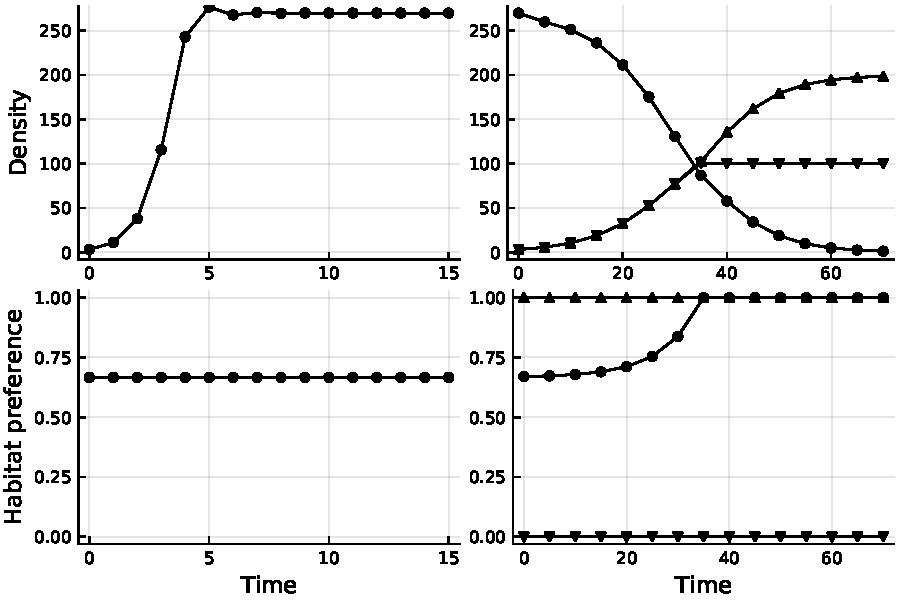
\includegraphics{figure02.pdf}
\caption{Population dynamics and habitat preference of the generalist
alone (left), and following invasion by the two specialists at the
generalist equilibrium (right). Circles represent the generalist, upper
and lower triangles represent the specialists of habitats 1 and 2
(respectively), and a diamond is used when both specialists have the
same behaviour.}\label{fig:02}
\end{figure}
}

In Fig. ~\ref{fig:03}, this implementation gives the same qualitative
results as the original article. There are small quantitative
differences in output, which are in my opinion explained by the initial
population densities (which are not given in the original article).
Absent variation in habitat quality, generalists cannot persist, and the
specialists both reach \(N^\star = \bar K\). There is a value of
variation for which the densities of specialists and generalists are
equal (about 110 for tied variations, and 130 for independent
variations).

\hypertarget{fig:03}{%
\begin{figure}
\centering
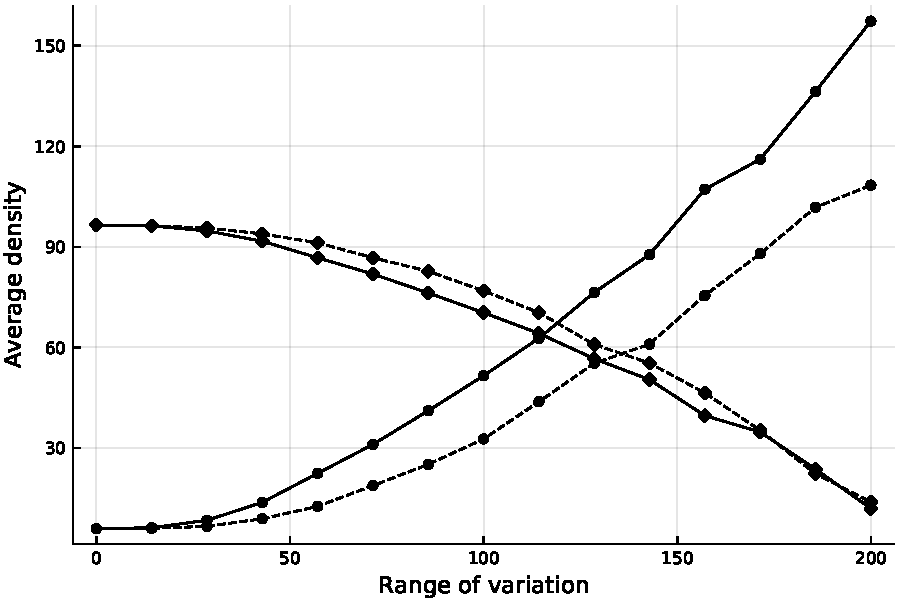
\includegraphics{figure03.pdf}
\caption{Consequences of increasing the range of variation of both
\(K_1\) and \(K_2\). Dashed lines represent independent variation, and
solid lines tied variations, as in the original article. Circles
represent the generalist, upper and lower triangles represent the
specialists of habitats 1 and 2 (respectively), and a diamond is used
when both specialists have the same behaviour.}\label{fig:03}
\end{figure}
}

In Fig. ~\ref{fig:04}, the same qualitative result (generalists increase
in abundance when one habitat becomes larger). The quantitative
differences can, again, be explained by changes in the initial
population densities. Finally, the results in Fig. ~\ref{fig:05} and
Fig. ~\ref{fig:06} can also be replicated; it should be noted that for
Fig. ~\ref{fig:06}, the lines cross at a different point, and diverge at
different rates, than in the original paper. Additional analyses suggest
that this depends on the number of timesteps used, as well as on the
starting populations. The original manuscript does not provides these
information, and so we will have to accept a \emph{qualitative}
replication of this result.

\hypertarget{fig:04}{%
\begin{figure}
\centering
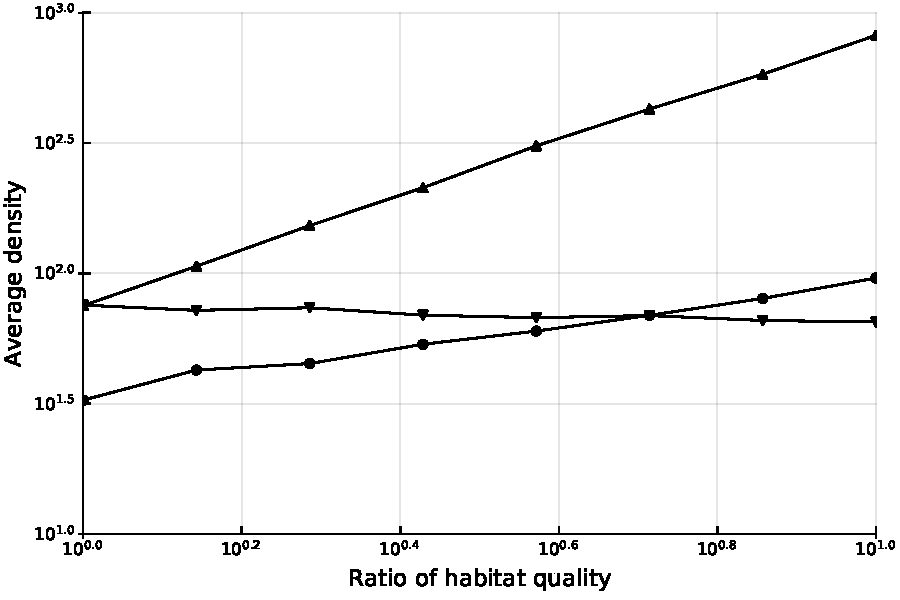
\includegraphics{figure04.pdf}
\caption{Consequences of changing the relative quality of habitats 1 and
2 on coexistence. Circles represent the generalist, upper and lower
triangles represent the specialists of habitats 1 and 2 (respectively),
and a diamond is used when both specialists have the same
behaviour.}\label{fig:04}
\end{figure}
}

\hypertarget{fig:05}{%
\begin{figure}
\centering
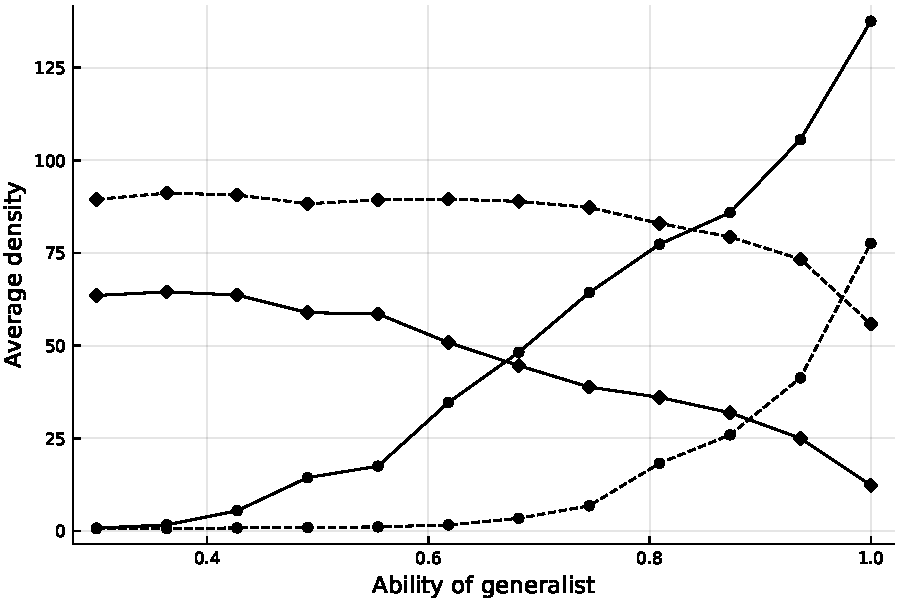
\includegraphics{figure05.pdf}
\caption{Consequences of changing \(b\), the ability of the generalist,
on coexistence. Dashed lines represent independent variation, and solid
lines tied variations, as in the original article. Circles represent the
generalist, upper and lower triangles represent the specialists of
habitats 1 and 2 (respectively), and a diamond is used when both
specialists have the same behaviour. Note that the direction of the axis
is \emph{reversed} with regard to the original figure.}\label{fig:05}
\end{figure}
}

\hypertarget{fig:06}{%
\begin{figure}
\centering
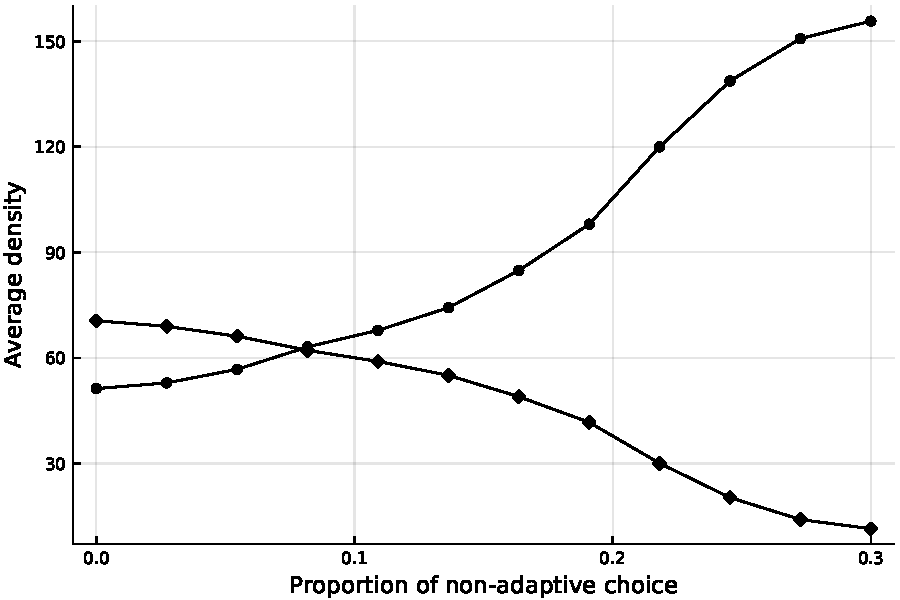
\includegraphics{figure06.pdf}
\caption{Consequences of changing the proportion of individuals picking
their habitat at random. Circles represent the generalist, upper and
lower triangles represent the specialists of habitats 1 and 2
(respectively), and a diamond is used when both specialists have the
same behaviour.}\label{fig:06}
\end{figure}
}

\hypertarget{conclusion}{%
\section{Conclusion}\label{conclusion}}

I believe that this implementation faithfully reproduces the results of
\textcite{wils94csg}. A single run of the model (using 100 generations
as in the original article) completes in
\(\approx 5\times 10^{-3} \text{s}\). This makes this implementation
usable for teaching, as it is not time consuming to generate results. As
an example, I merged the output of Fig. ~\ref{fig:03} and Fig.
~\ref{fig:05}, to generate the response of Pielou's evenness
\autocite{piel66sps},

\[
J' = -\left(\sum_{i=1}^3\frac{N_i}{N}\text{ln}\frac{N_i}{N}\right)\frac{1}{\text{ln}\,3} \,,
\]

which measures the extent to which all species have the same density. It
appears that \(J'\), a measure of coexistence, changes in response to
both the rate of variation \emph{and} generalist ability. The results
are presented in Fig. ~\ref{fig:surf}. This figure is primarily intended
to show that this model can still generate new insights when we vary
multiple parameters: namely, the response of equitability to changes in
multiple variables is non-linear, and maximum equitability is reach for
high generalist ability but moderate range of variation (this was not
predictable from the outputs of Figs. ~\ref{fig:04} and ~\ref{fig:05}
alone).

\hypertarget{fig:surf}{%
\begin{figure}
\centering
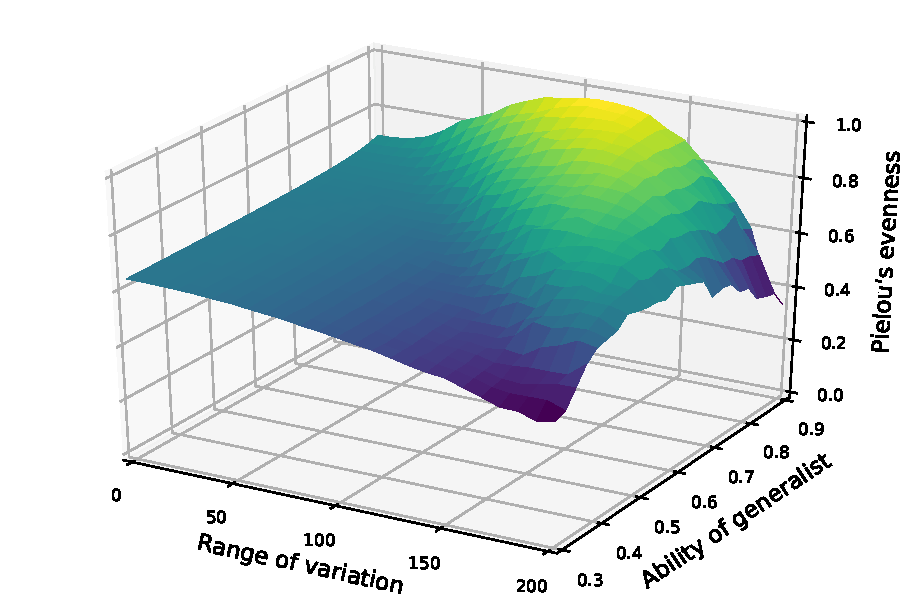
\includegraphics{figureSurf.pdf}
\caption{Response of the model to changing the ability of the generalist
\emph{and} the range of variation. While the response to environmental
change is hump-shaped when generalists are competitive (\(b\) close to
unity), it becomes monotonously decreasing for generalists with lower
competitive ability (\(b\) close to \(a\)).}\label{fig:surf}
\end{figure}
}

{\sffamily \small
  \printbibliography[title=References]
}
\end{document}
